\documentclass[../../eatbrain.tex]{subfile}
La pagina Events raccoglie pregi e difetti scritti in precedenza (come i link di difficile individuazione, sono scritte bianche) e presenta un \textbf{What} ben congegnato: gli eventi sono disposti a mo di lista ed è presente la categorizzazione tra eventi passati ed eventi futuri. \\
L'\textbf{How} presenta lo stesso problema delle altre pagina ma peggiora togliendo la possibilità di effettuare la ricerca via browser: in presenza ti tanti eventi, per motivi di prestazioni e tempi di caricamento, questi non vengono caricati tutti nell'immediato ma è presente un tasto "Load More" per caricare i restati. Questa accortezza elimina la possibilità di effettuare la ricerca via browser: per eventi posti troppo indietro nel passato o troppo avanti nel futuro sono necessarie diverse iterazioni per raggiungere l'informazione cercata. \\
In più il tasto "Load More" appare come una semplice scritta di testo e non è riconoscibile nell'immediato. \\
Ultima pecca è nei link: questi reindirizzano all'evento Facebook senza mostrare alcun avvertimento, come già detto nelle sezioni precedenti questo comportamento può causare confusione nell'utente.
\begin{figure}[h]
	\centering
	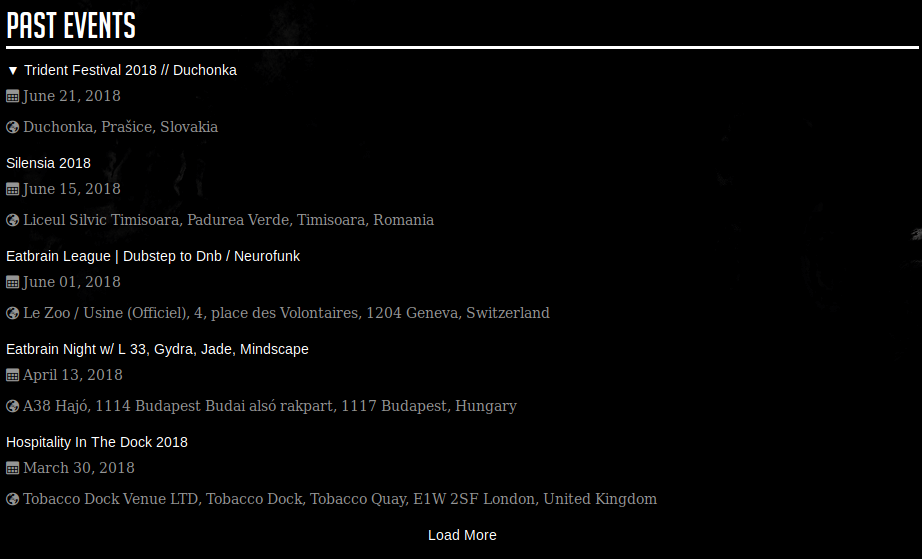
\includegraphics[width=12cm]{immagini/events}
	\caption{Snapshot della pagina Events e tasto "Load More" incriminato}
	\label{img-events}
\end{figure}